\documentclass[garamond]{goose-article}

\hypersetup{pdfauthor={T.W.J. de Geus}}

\title{Linear elasticity}

\author[1]{Tom de Geus}

%\affil[1]{} % use '\nl' for line-breaks

%\contact{}

%\header{}
%\headerEven{}
%\headerOdd{}

\begin{document}

\maketitle

%\begin{abstract}
%\end{abstract}

%\keywords{}

\section{Consistency check}

To check if the derived tangent $\mathbb{C}$ a \emph{consistency check} can be performed. A (random) perturbation $\delta \bm{\varepsilon}$ is applied. The residual is compared to that predicted by the tangent. For the linearisation, the following holds:
%
\begin{equation}
  \bm{\sigma}\big( \bm{\varepsilon}_\star + \delta \bm{\varepsilon} \big) =
  \bm{\sigma}\big( \bm{\varepsilon}_\star \big) +
  \mathbb{C} \big( \bm{\varepsilon}_\star \big) : \delta \bm{\varepsilon} +
  \mathcal{O}(\delta \bm{\varepsilon}^2)
\end{equation}
%
or
%
\begin{equation}
  \underbrace{
    \bm{\sigma}\big( \bm{\varepsilon}_\star + \delta \bm{\varepsilon} \big) -
    \bm{\sigma}\big( \bm{\varepsilon}_\star \big)
  }_{
    \displaystyle \delta \bm{\sigma}
  } -
  \mathbb{C} \big( \bm{\varepsilon}_\star \big) : \delta \bm{\varepsilon} =
  \mathcal{O}(\delta \bm{\varepsilon}^2)
\end{equation}
%
This allows us the introduction of a relative error
%
\begin{equation}
  \eta =
  \Big|\Big|
    \delta \bm{\sigma} -
    \mathbb{C}(\bm{\varepsilon}_\star) : \delta \bm{\varepsilon}
  \Big|\Big|
  /
  \Big|\Big| \delta \bm{\sigma} \Big|\Big|
\end{equation}
%
Because of the first order accuracy of the linearization, the error should scale linearly with the amplitude of the strain perturbation. This can be shown in a graph such as Figure~\ref{fig:newton:consistency}. The expected behavior is found in the right hand side of the graph, denoted as \textit{truncation error}. Also visible in this graph is that once the amplitude of the strain perturbation becomes sufficiently small, $10^{-8}$ to be exact, numerical errors become dominant, causing the error $\eta$ to increase again.

\begin{figure}[htp]
  \centering
  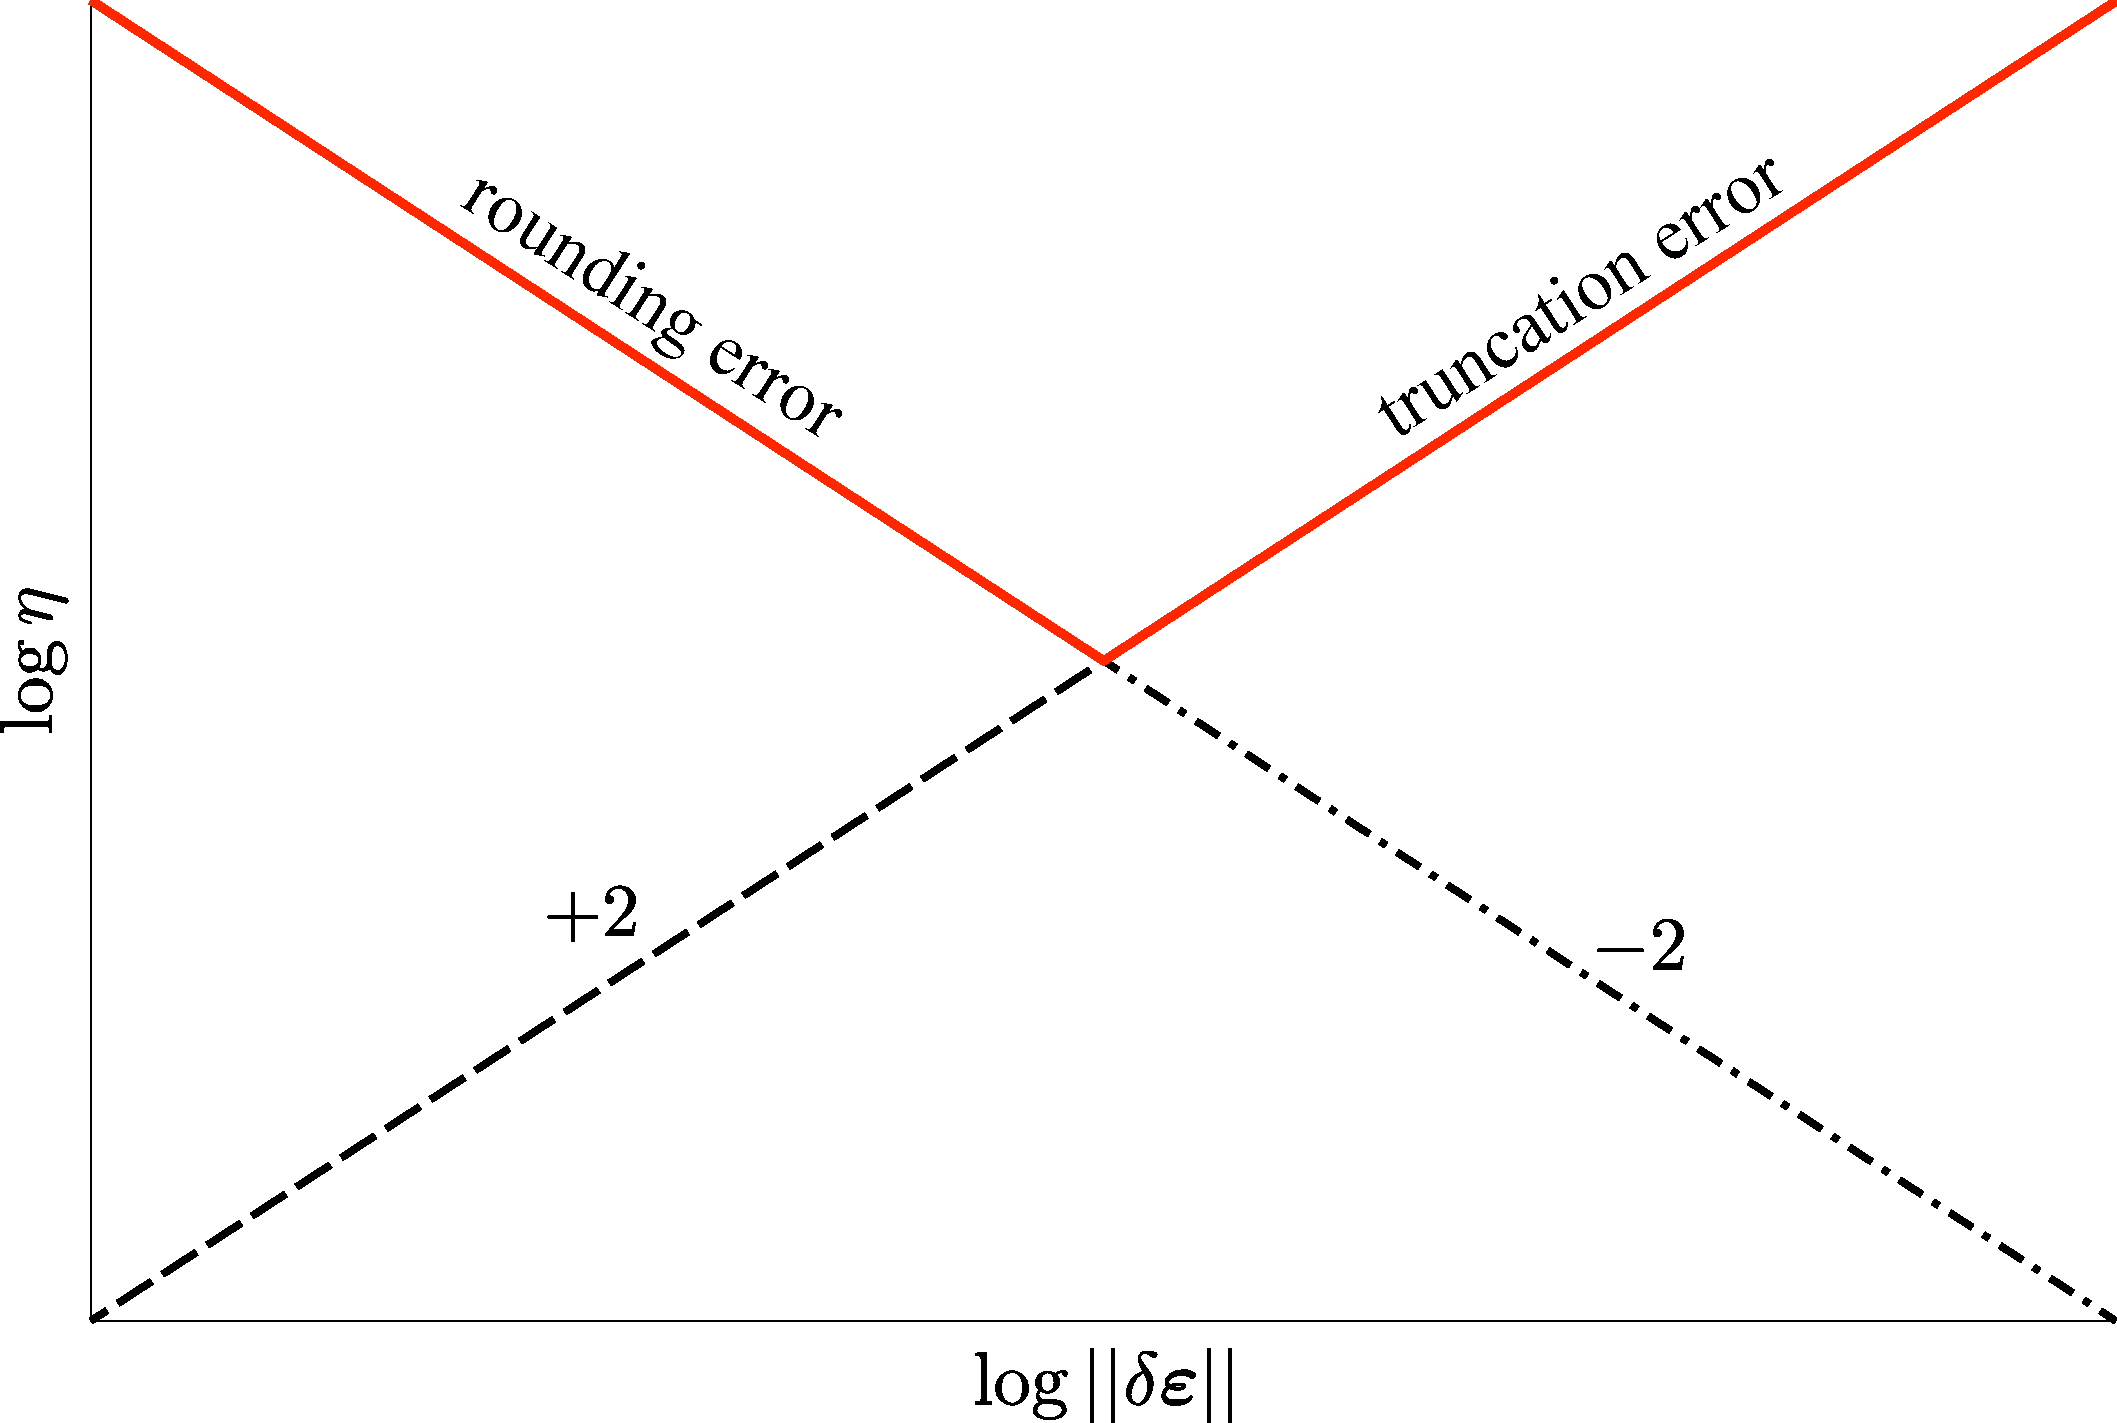
\includegraphics[width=.5\textwidth]{figures/consistency}
  \caption{Expected behaviour of the consistency check, see \citet[p.~9]{Heath2002}.}
  \label{fig:newton:consistency}
\end{figure}

\bibliography{library}

\end{document}
